\documentclass[10pt,twocolumn]{article}
\usepackage{lmodern,setspace,amsmath,amssymb,amsfonts,amsthm,graphicx,multicol,grffile}
\usepackage[top=0.9in, bottom=1.15in, left=1.15in, right=1.25in]{geometry}
\usepackage[polish]{babel}
\usepackage[utf8]{inputenc}
\usepackage[T1]{fontenc}
\title{Algorytmy i struktury danych - Sortowanie}
\author{Dariusz Max Adamski}
\date{Poznań, 20.03.2018}

\begin{document}

\maketitle

W tym sprawozdaniu porównywana będzie efektywność różnych algorytmów sortujących, w odniesieniu do ich złożoności obliczeniowej, zużycia pamięci i czasu wykonywania. Brane pod uwagę będą także przypadki krańcowe, czyli dane wejściowe, dla których algorytm może mieć zdecydowanie dłuższy czas wykonywania, niż dla ciągu złożonego z liczb losowych, generowanych zgodnie z równomiernym rozkładem prawdopodobieństwa.

Dla odniesienia, na wykresach zostały także umieszczone czasy dla algorytmu sortowania z biblioteki standardowej języka C++.

Pierwszymi porównywanymi algorytmami będą sortowanie bąbelkowe (BS), sortowanie stogowe (HS), sortowanie przez zliczanie (CS) oraz sortowanie Shella (ShS). Czasy wykonywania są przedstawione na wykresach \ref{los_bub}, \ref{los} i \ref{los_bub_log}.

\begin{figure}[h!]
	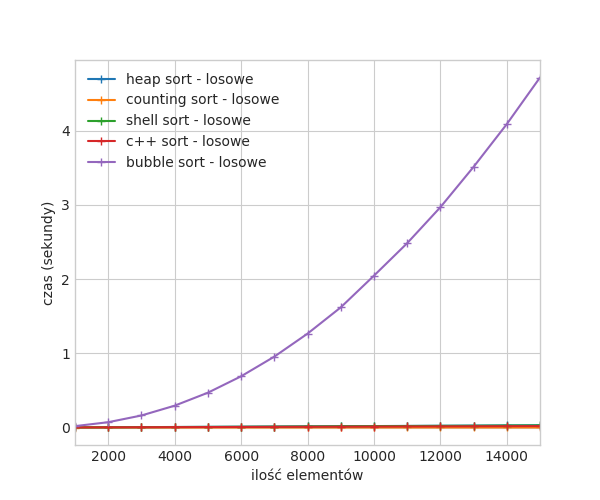
\includegraphics[width=\linewidth]{plots/los_bub.png}
	\caption{Czas sortowania losowych danych \label{los_bub}}
\end{figure}

Sortowanie bąbelkowe to algorytm o złożoności obliczeniowej $O(n^2)$ [\ref{los_bub}]. Dla danych losowych, w porównaniu z algorytmami HS, CS i ShS, sortowanie bąbelkowe zajmuje najwięcej czasu. Ponieważ, przy tablich o liczbie elementów większej niż 1000, skala czasu bardzo się wydłuża, algorytmy o złożoności $O(n \log n)$ zostały porównane na wykresie \ref{los}.

Algorytmy sortowania stogowego, przez zliczanie i Shella to algorytmy o złożoności obliczeniowej $O(n \log n)$

\begin{figure}[h!]
	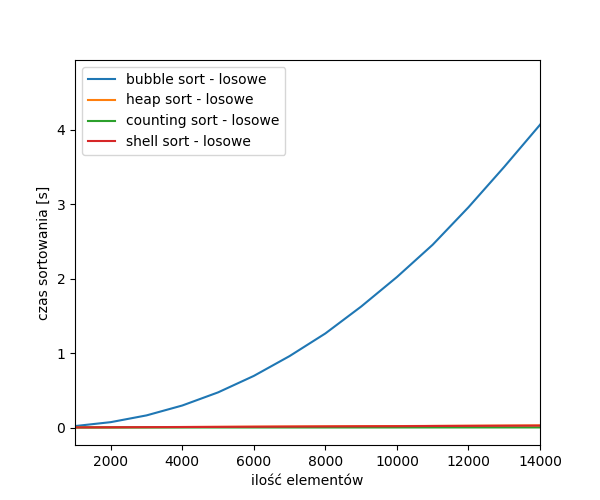
\includegraphics[width=\linewidth]{plots/los.png}
	\caption{Czas sortowania losowych danych \label{los}}
\end{figure}

\begin{figure}[h!]
	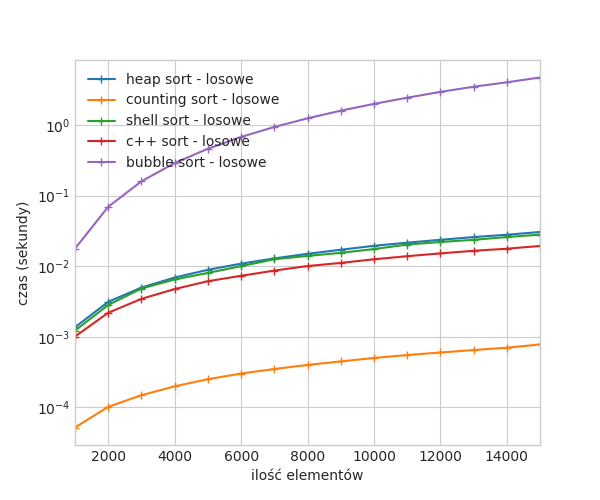
\includegraphics[width=\linewidth]{plots/los_bub_log.png}
	\caption{Czas sortowania losowych danych ()\label{los_bub_log}}
\end{figure}

Officiis ducimus ipsum quidem perferendis labore qui. Reprehenderit assumenda hic ea ullam dolor tempore et ut. Saepe dolore cumque id est alias rerum consequatur animi. Quam nulla illum amet fugit non natus vel sint [\ref{los}].

\begin{figure}
	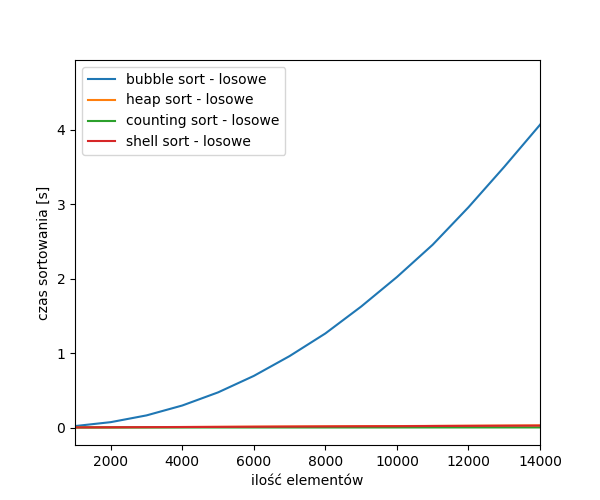
\includegraphics[width=\linewidth]{plots/los.png}
	\caption{Czas sortowania losowych danych (skala logarytmiczna) \label{los_log}}
\end{figure}

Officia eligendi tempora non consequatur magnam quo tenetur. Eveniet sunt minima aliquam autem tempore quod. Ut numquam sint quaerat dolorem ex et. Totam excepturi et earum ipsam consequatur nihil quae autem. Voluptatem ut animi est. Dicta explicabo dolorem aut unde maiores sit [\ref{los_log}].

\begin{figure}[h!]
	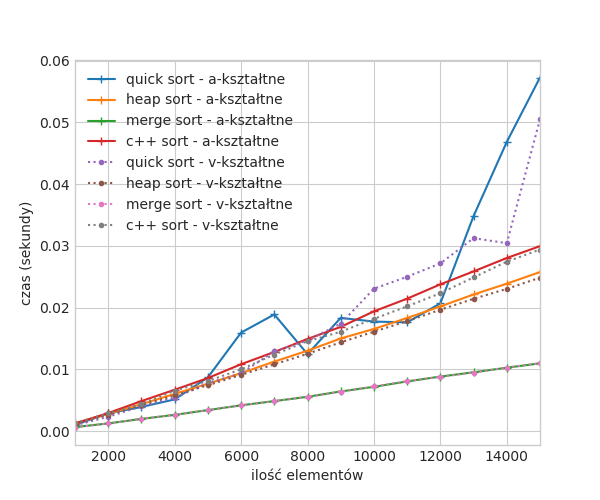
\includegraphics[width=\linewidth]{plots/av.png}
	\caption{Efektywność sortowania danych a-kształtnych i v-kształtnych \label{aksz_vksz}}
\end{figure}

Quis aliquid atque ut id explicabo omnis. Sequi aperiam earum quo. Dicta aut velit est repudiandae consequatur. Facilis laudantium molestiae consequatur qui officia. Voluptas debitis velit id quasi. Sint tenetur est quo cum.

\begin{figure}[h!]
	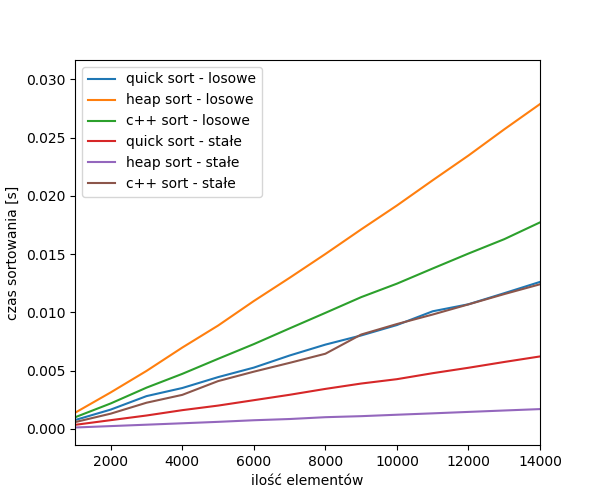
\includegraphics[width=\linewidth]{plots/ls.png}
	\caption{Efektywność sortowania danych losowych i stałych \label{los_sta}}
\end{figure}

Kuis aliquid atque ut id explicabo omnis. Sequi aperiam earum quo. Dicta aut velit est repudiandae consequatur. Facilis laudantium molestiae consequatur qui officia.

\begin{figure}[h!]
	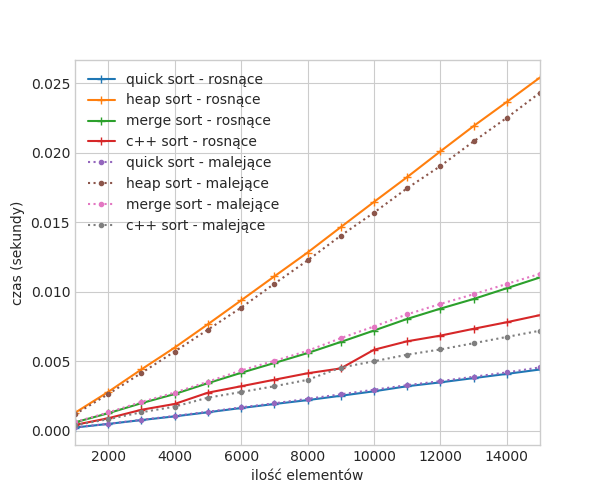
\includegraphics[width=\linewidth]{plots/rm.png}
	\caption{Czas sortowania danych rosnących i malejących \label{ros_mal}}
\end{figure}

Quasi consequuntur itaque qui aliquam dolorem reprehenderit quos ut. Quis recusandae accusamus amet sint expedita perspiciatis sint. Debitis est et id tempora rerum. Blanditiis quam dolorem quia.

\end{document}

